%  LaTeX support: latex@mdpi.com 
%  In case you need support, please attach all files that are necessary for compiling as well as the log file, and specify the details of your LaTeX setup (which operating system and LaTeX version / tools you are using).

%=================================================================
\documentclass[journal,article,submit,moreauthors,pdftex]{Definitions/mdpi} 

\usepackage{booktabs} % For formal tables
\usepackage{array}
\usepackage{multirow}
\usepackage{subcaption}
\newcommand{\emad}[1]{\textcolor{red}{{\it [Emad: #1]}}}
\newcommand{\hosein}[1]{\textcolor{orange}{{\it [Hosein: #1]}}}
\newcommand{\todo}[1]{\colorbox{yellow}{\textbf{[#1]}}}

% If you would like to post an early version of this manuscript as a preprint, you may use preprint as the journal and change 'submit' to 'accept'. The document class line would be, e.g., \documentclass[preprints,article,accept,moreauthors,pdftex]{mdpi}. This is especially recommended for submission to arXiv, where line numbers should be removed before posting. For preprints.org, the editorial staff will make this change immediately prior to posting.

%--------------------
% Class Options:
%--------------------
%----------
% journal
%----------
% Choose between the following MDPI journals:
% acoustics, actuators, addictions, admsci, aerospace, agriculture, agriengineering, agronomy, algorithms, animals, antibiotics, antibodies, antioxidants, applsci, arts, asc, asi, atmosphere, atoms, axioms, batteries, bdcc, behavsci , beverages, bioengineering, biology, biomedicines, biomimetics, biomolecules, biosensors, brainsci , buildings, cancers, carbon , catalysts, cells, ceramics, challenges, chemengineering, chemistry, chemosensors, children, cleantechnol, climate, clockssleep, cmd, coatings, colloids, computation, computers, condensedmatter, cosmetics, cryptography, crystals, dairy, data, dentistry, designs , diagnostics, diseases, diversity, drones, econometrics, economies, education, electrochem, electronics, energies, entropy, environments, epigenomes, est, fermentation, fibers, fire, fishes, fluids, foods, forecasting, forests, fractalfract, futureinternet, futurephys, galaxies, games, gastrointestdisord, gels, genealogy, genes, geohazards, geosciences, geriatrics, hazardousmatters, healthcare, heritage, highthroughput, horticulturae, humanities, hydrology, ijerph, ijfs, ijgi, ijms, ijtpp, informatics, information, infrastructures, inorganics, insects, instruments, inventions, iot, j, jcdd, jcm, jcp, jcs, jdb, jfb, jfmk, jimaging, jintelligence, jlpea, jmmp, jmse, jnt, jof, joitmc, jpm, jrfm, jsan, land, languages, laws, life, literature, logistics, lubricants, machines, magnetochemistry, make, marinedrugs, materials, mathematics, mca, medicina, medicines, medsci, membranes, metabolites, metals, microarrays, micromachines, microorganisms, minerals, modelling, molbank, molecules, mps, mti, nanomaterials, ncrna, neonatalscreening, neuroglia, nitrogen, notspecified, nutrients, ohbm, particles, pathogens, pharmaceuticals, pharmaceutics, pharmacy, philosophies, photonics, physics, plants, plasma, polymers, polysaccharides, preprints , proceedings, processes, proteomes, psych, publications, quantumrep, quaternary, qubs, reactions, recycling, religions, remotesensing, reports, resources, risks, robotics, safety, sci, scipharm, sensors, separations, sexes, signals, sinusitis, smartcities, sna, societies, socsci, soilsystems, sports, standards, stats, surfaces, surgeries, sustainability, symmetry, systems, technologies, test, toxics, toxins, tropicalmed, universe, urbansci, vaccines, vehicles, vetsci, vibration, viruses, vision, water, wem, wevj

%---------
% article
%---------
% The default type of manuscript is "article", but can be replaced by: 
% abstract, addendum, article, benchmark, book, bookreview, briefreport, casereport, changes, comment, commentary, communication, conceptpaper, conferenceproceedings, correction, conferencereport, expressionofconcern, extendedabstract, meetingreport, creative, datadescriptor, discussion, editorial, essay, erratum, hypothesis, interestingimages, letter, meetingreport, newbookreceived, obituary, opinion, projectreport, reply, retraction, review, perspective, protocol, shortnote, supfile, technicalnote, viewpoint
% supfile = supplementary materials

%----------
% submit
%----------
% The class option "submit" will be changed to "accept" by the Editorial Office when the paper is accepted. This will only make changes to the frontpage (e.g., the logo of the journal will get visible), the headings, and the copyright information. Also, line numbering will be removed. Journal info and pagination for accepted papers will also be assigned by the Editorial Office.

%------------------
% moreauthors
%------------------
% If there is only one author the class option oneauthor should be used. Otherwise use the class option moreauthors.

%---------
% pdftex
%---------
% The option pdftex is for use with pdfLaTeX. If eps figures are used, remove the option pdftex and use LaTeX and dvi2pdf.

%=================================================================
\firstpage{1} 
\makeatletter 
\setcounter{page}{\@firstpage} 
\makeatother
\pubvolume{xx}
\issuenum{1}
\articlenumber{5}
\pubyear{2019}
\copyrightyear{2019}
%\externaleditor{Academic Editor: name}
\history{Received: date; Accepted: date; Published: date}
%\updates{yes} % If there is an update available, un-comment this line

%% MDPI internal command: uncomment if new journal that already uses continuous page numbers 
%\continuouspages{yes}

%------------------------------------------------------------------
% The following line should be uncommented if the LaTeX file is uploaded to arXiv.org
%\pdfoutput=1

%=================================================================
% Add packages and commands here. The following packages are loaded in our class file: fontenc, calc, indentfirst, fancyhdr, graphicx, lastpage, ifthen, lineno, float, amsmath, setspace, enumitem, mathpazo, booktabs, titlesec, etoolbox, amsthm, hyphenat, natbib, hyperref, footmisc, geometry, caption, url, mdframed, tabto, soul, multirow, microtype, tikz

%=================================================================
%% Please use the following mathematics environments: Theorem, Lemma, Corollary, Proposition, Characterization, Property, Problem, Example, ExamplesandDefinitions, Hypothesis, Remark, Definition
%% For proofs, please use the proof environment (the amsthm package is loaded by the MDPI class).

%=================================================================
% Full title of the paper (Capitalized)
\Title{Impact of Featureset on Cross-Trials and Cross-Subjects Evaluation for Human Activity Recognition }

% Author Orchid ID: enter ID or remove command
\newcommand{\orcidauthorA}{0000-0000-000-000X} % Add \orcidA{} behind the author's name
%\newcommand{\orcidauthorB}{0000-0000-000-000X} % Add \orcidB{} behind the author's name

% Authors, for the paper (add full first names)
\Author{Hosein Nourani $^{1,\dagger,\ddagger}$\orcidA{}, Emad Shihab $^{1,\ddagger}$ and Omid Sarbishei $^{2,}$*}

% Authors, for metadata in PDF
\AuthorNames{Hosein Nourani, Emad Shihab and Omid Sarbishei}

% Affiliations / Addresses (Add [1] after \address if there is only one affiliation.)
\address{%
$^{1}$ \quad Dept. of Computer Science and Software Engineering; h$.$nourani@hotmail.com\\
$^{2}$ \quad Dept. of Computer Science and Software Engineering; e$.$shihab@concordia.com}

% Contact information of the corresponding author
\corres{Correspondence: e-mail@e-mail.com; Tel.: (optional; include country code; if there are multiple corresponding authors, add author initials) +xx-xxxx-xxx-xxxx (F.L.)}

% Current address and/or shared authorship
\firstnote{Current address: Affiliation 3} 
\secondnote{These authors contributed equally to this work.}
% The commands \thirdnote{} till \eighthnote{} are available for further notes

%\simplesumm{} % Simple summary

%\conference{} % An extended version of a conference paper

% Abstract (Do not insert blank lines, i.e. \\) 
\abstract{Human Activity Recognition (HAR) refers to an emerging area of interest for medical, military, and security applications. However, the identification of the features to be used for activity classification and recognition is still an open point. In this work we have compared several state-of-the-art featuresets on HAR. To compare the featuresets, we have conducted an extensive set of experiments to indicate the vulnerable points in using featuresets. Aiming this goal, we implement several state-of-the-art machine learning models, ranging from traditional classifiers like SVM and GLM to convolutional neural networks; the models get evaluated by the performance gained using two challenging evaluation methods including cross-trials evaluation and cross-subjects evaluation, in addition to the convention method of 10-fold validation. The data from 55 gym exercises performing by thirteen subject have been recorded. To keep the realistic condition, they were asked to perform based on their own practice program. To capture the movements, two IMUs have been attached to the right wrist and right foot of the subjects. In total, 1300 features were extracted from the data. Our results showed that FNN acheived the highest performances using different featuresets. Against the prevailing wisdom, the statistical features gets outperformed by histogram feature set to deliver the best performance under all evaluation methods. 
	%(1) Background: Place the question addressed in a broad context and highlight the purpose of the study; (2) Methods: Describe briefly the main methods or treatments applied; (3) Results: Summarize the article's main findings; and (4) Conclusion: Indicate the main conclusions or interpretations. The abstract should be an objective representation of the article, it must not contain results which are not presented and substantiated in the main text and should not exaggerate the main conclusions.
}

% Keywords
\keyword{feature selection; featureset; Wearable; Motion sensor; Neural Network, Histogram, Human activity recognition }

% The fields PACS, MSC, and JEL may be left empty or commented out if not applicable
%\PACS{J0101}
%\MSC{}
%\JEL{}

%%%%%%%%%%%%%%%%%%%%%%%%%%%%%%%%%%%%%%%%%%
% Only for the journal Diversity
%\LSID{\url{http://}}

%%%%%%%%%%%%%%%%%%%%%%%%%%%%%%%%%%%%%%%%%%
% Only for the journal Applied Sciences:
%\featuredapplication{Authors are encouraged to provide a concise description of the specific application or a potential application of the work. This section is not mandatory.}
%%%%%%%%%%%%%%%%%%%%%%%%%%%%%%%%%%%%%%%%%%

%%%%%%%%%%%%%%%%%%%%%%%%%%%%%%%%%%%%%%%%%%
% Only for the journal Data:
%\dataset{DOI number or link to the deposited data set in cases where the data set is published or set to be published separately. If the data set is submitted and will be published as a supplement to this paper in the journal Data, this field will be filled by the editors of the journal. In this case, please make sure to submit the data set as a supplement when entering your manuscript into our manuscript editorial system.}

%\datasetlicense{license under which the data set is made available (CC0, CC-BY, CC-BY-SA, CC-BY-NC, etc.)}

%%%%%%%%%%%%%%%%%%%%%%%%%%%%%%%%%%%%%%%%%%
% Only for the journal Toxins
%\keycontribution{The breakthroughs or highlights of the manuscript. Authors can write one or two sentences to describe the most important part of the paper.}

%\setcounter{secnumdepth}{4}
%%%%%%%%%%%%%%%%%%%%%%%%%%%%%%%%%%%%%%%%%%
\begin{document}
%%%%%%%%%%%%%%%%%%%%%%%%%%%%%%%%%%%%%%%%%%

%%%%%%%%%%%%%%%%%%%%%%%%%%%%%%%%%%%%%%%%%%
%The order of the section titles is: Introduction, Materials and Methods, Results, Discussion, Conclusions for these journals: aerospace,algorithms,antibodies,antioxidants,atmosphere,axioms,biomedicines,carbon,crystals,designs,diagnostics,environments,fermentation,fluids,forests,fractalfract,informatics,information,inventions,jfmk,jrfm,lubricants,neonatalscreening,neuroglia,particles,pharmaceutics,polymers,processes,technologies,viruses,vision

\section{Introduction}

%The introduction should briefly place the study in a broad context and highlight why it is important. It should define the purpose of the work and its significance. The current state of the research field should be reviewed carefully and key publications cited. Please highlight controversial and diverging hypotheses when necessary. Finally, briefly mention the main aim of the work and highlight the principal conclusions. As far as possible, please keep the introduction comprehensible to scientists outside your particular field of research. Citing a journal paper \cite{ref-journal}. And now citing a book reference \cite{ref-book}. Please use the command \citep{ref-journal} for the following MDPI journals, which use author-date citation: Administrative Sciences, Arts, Econometrics, Economies, Genealogy, Humanities, IJFS, JRFM, Languages, Laws, Religions, Risks, Social Sciences.
%%%%%%%%%%%%%%%%%%%%%%%%%%%%%%%%%%%%%%%%%%
Human Activity Recognition (HAR) using inertial sensors has been a target of a lot of researches in the last decade. one reason is because it opens a door to the thousands of useful applications in healthcare, physical fitness monitoring, elder care support and etc. Another reason is due to the pervasiveness of wearable sensors. They are small in size, cheap, and already embedded in almost all wearable gadgets. This is a promising point for HAR applications since no extra hardware setup-cost is required for users to start using them immediately. This is to say that the most challenging part in HAR is to producing an application to be able to efficiently use the device's resources and deliver the most accurate result in the form of classifying the activity type or counting it \cite{schilit1994context}.\\
Basically, a HAR system using Inertial Measurement Units (IMUs) is composed of two basic components: (1) a data acquisition unit responsible for capturing human movements, (2) a processing unit responsible for recognizing the certain activities among movements of the subject\cite{rosati2018comparison}. In the first component, the human movements is captured by different motion sensors such as accelerometer, gyroscope, and so on. These sensors can be located in an off-the-shelf device like a smart-phone for general HAR applications or specifically are accompanied by a storage and a processor, formed a System on Chip (SoC) for a certain purpose.\\
The captured movements as raw data transmits to the second component for processing operation. Within this component, there is a pattern recognition (HAR) model that classifies the input signals into certain classes of activities. This HAR model typically consists of three phases. First, there is a pre-processing operation that extracts informative features from raw signal. Second, a classifier is trained over extracted features. Third, an evaluation method to ensure that the classifier provides the required performance\cite{kolodziej2019registration}. In other words, a HAR model should address these three aspects to be able to recognize an activity. The previous studies have achieved many improvements in each stages[][][] however there are challenging aspects that they did not contemplate them and they are still open:
\begin{itemize}[leftmargin=*,labelsep=5.8mm]
	\item	Identifying the correct set of input features for the classifier\cite{rosati2018comparison} (in the phase 1)
	\item	Existing an unique and reliable validation protocol to assess the models \cite{jordao2018human}(in the phase 3)
\end{itemize} 
%(3) impact of quality of dataset on performance since they vary from paper to paper\cite{jordao2018human}.\\
%While the first two issues have impact on performance of a model in general, the third one influences directly on recognition result, independent from how much a model is well designed. Factors like size of dataset, frequency rate of sensors, complexity of target activities, sensor position and how it is attached to the body, and so on. In [], the authors, looking for impact of sensor alignments, in two different trials attached the sensor to the subjects. In first trial, an expert attached the sensor while in the second trial, subjects were asked to attached the sensors by themselves. Results show that the performance has a significant collapse during the second trials.
%
While the first issue plays an important role to improve the performance of the model, the second issue is a critical point since different validation methods show the performance differently, somehow biased. For the same reason, using HAR models on new dataset shows a significant decrease in performance. As a consequence of this issue, currently it is impossible to know the state-of-the-art methods in human activity recognition\cite{jordao2018human}. Addition to this, some factors like temporal changes in user body (e.g., tiredness) have impacts on how they perform an identical activity within two different trials. However, it is impossible to evaluate such impacts by using the the traditional validation methods like k-fold cross-validation or Leave-One-Subject-Out (LOSO). To address this issue, in this study, we employ Leave-One-Trial-Out (LOTO) cross-validation addition to conventional validation methods. Using this validation method, we show that how the performance and robustness of the model change by feeding it by more trials.\\
Regarding the first issue, previous works have employed a wide range of features for HAR model. Dealing with selecting appropriate features for a HAR model (feature selection methods) are usually aiming to improve the performance of the model. However in \cite{rosati2018comparison} which is the most similar previous work to us, the authors also listed three extra issues which less have been considered in previous works:
(1) The processing cost of producing a feature
(2) The complexity of calculation of features makes a model difficult to understand.
(3) The negative impacts of having too much number of features on performance of the model.
In our previous work\cite{Nourani_CoMoRea2019}, we showed that by removing redundant features, we can keep the performance identical while shrink the dataset to 8\% of its initial size. This approach significantly decreases the processing cost and vulnerability of getting overfit. In this study, we will focus on decreasing \textbf{the complexity of calculation of features} rather just decreasing size of dataset in a feature-set.\\

The aforementioned discussion motivated our study, where we evaluate a wide range of features by the performance reached by six popular classifiers. The models train and evaluate on two huge datasets (include our dataset which is one of the biggest dataset on gym exercises, publicly available). To provide a more robust evaluation we validate our models under several cross-validation methods.

The aim of this article is to present the following main contributions:
\begin{itemize}
	\item Implementation and evaluation of the remarkable state-of-the-art featuresets.
	\item Analysing the impact of temporal changes on HAR model.
	\item Proposition of a novel model using Forward Neural Network (FNN) in HAR
\end{itemize}
Regarding the target datasets, we chose [] dataset since it provides a wide range of activities (33 activities) and it is big enough. However, to the best of our knowledge, there is no dataset that targets different trials of same activity with same subject, publicly available. So, we collected a dataset of 15 subjects and +50 gym activities including different trials for each activity.

The rest of this paper is organized as follows. Section 2 describes the study setup including the approach and the dataset used in this study. Section 3 defines the featuresets and theirs advantages in previous works. Section 4 presents the results of using featuresets on classifiers. Finally, Section 7 summarizes this study and highlight the most important contributions of this paper for future works.
\section{Related Work}
To the best of our knowledge, the statistical functions on time-domain signal provide the most popular features in HAR. Features like mean, median, mean standard deviation, variance, minimum, maximum are the most popular ones. The second group, Frequency-domain features are so helpful for those models that target periodic activities like walking. To achieve a frequency-domain feature, one segment of time signal should be transferred to several components in frequency domain. Each component may/may not have meaning depend on the activity. Frequency bins and auto-correlation coefficient are some example.

Suto et al., 2017 investigate the efficiency of the popular machine learning strategies based on a right-ankle-mounted accelerometer, and their results suggest that one sensor is not enough for appropriate daily activity recognition due to the similar data generated from one sensor for different activities
Generally, One to One is the basic deployment and more suitable for the basic recognition tasks, such as step counting or sleep quality monitoring
Placing more sensors on multiple body parts is intuitively beneficial for improving the performance and robustness, whereas this can also result in increased complexity in deployment and computation cost
Sztyler et al., 2017 develop a position-aware HAR system by placing seven accelerometers in different body positions
\section{Data}

\subsection{Signal Acquisition}
Real-world data is the first material and crucial for the recognition tasks after determining sensor types and
sensor deployment
In this work, we have employed a SoC device which called \textit{Neblina}.
\subsubsection{Neblina}  Neblina is a miniature-sized box containing three tri-axial motion sensors (accelerometer, gyroscope, magnetometer) along with a processor, a flash memory, battery, and a bluetooth port. Using blue-tooth port, it can transmit the result to a host (e.g., cellphone or desktop computer).  In fact, Neblina is equipped with all requirements for a real-time HAR system. Comparing with a smartphone, Neblina is much smaller (Figure \ref{neblina_setup}) that lets us to attach it to different part of the subject's body without making any interrupt in his/her actions\cite{de2018comparative}. Having access directly to different resources like sensors or memory without OS interferences is another advantage of using Neblina that let us improve the efficiency of the model.
\begin{figure}[H]
	\centering
	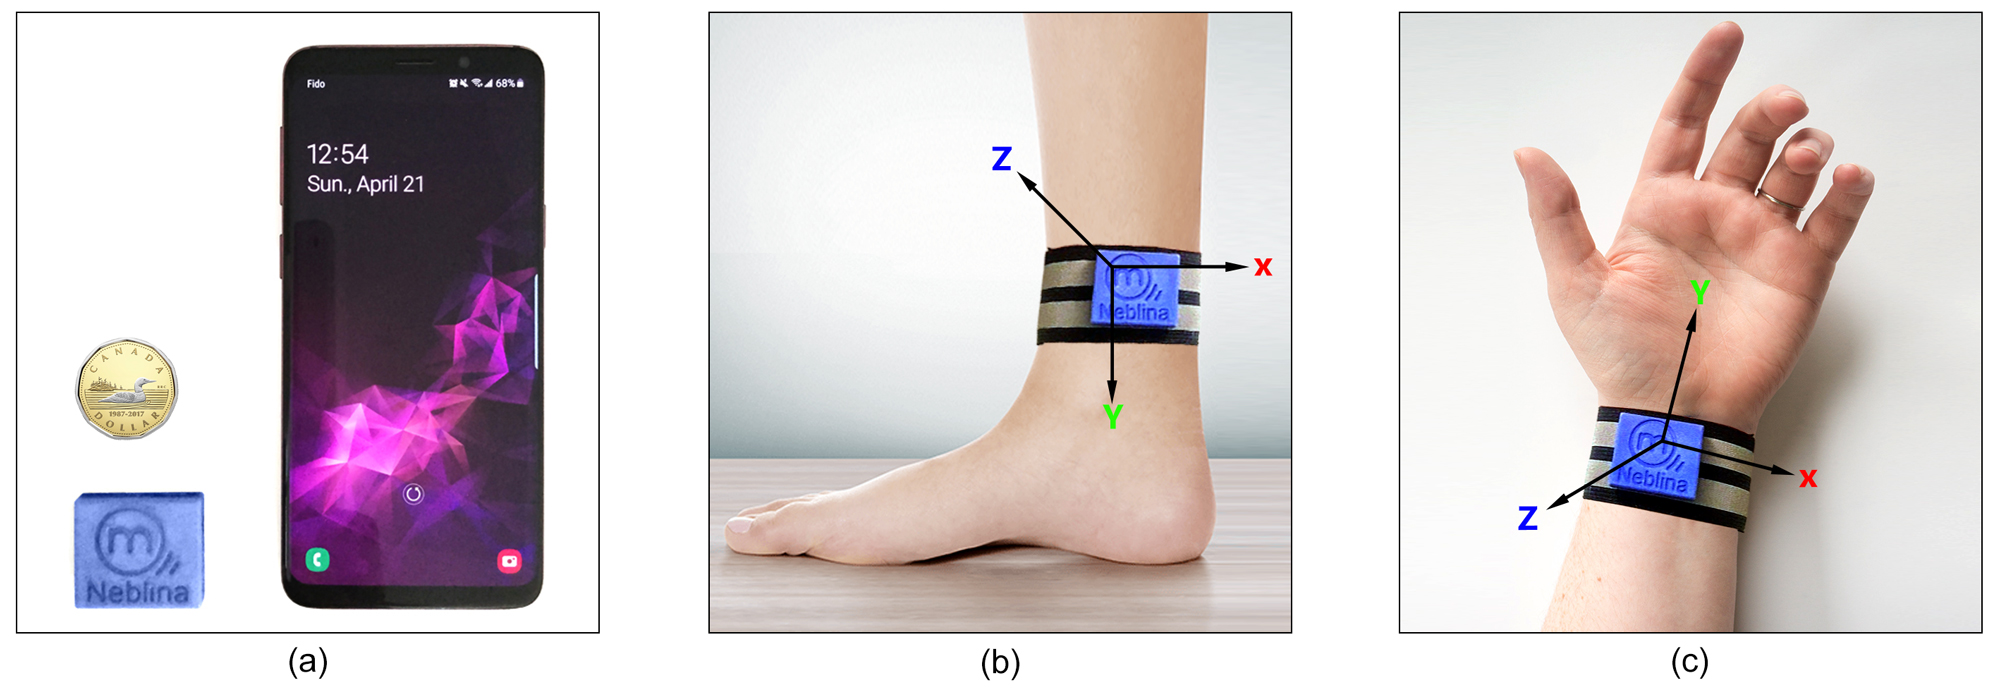
\includegraphics[width=10 cm]{Definitions/images/neblina_setup.jpg}
	\caption{Neblina setup. (a) Compares dimensions of Neblina with a 1 dollar coin and a cellphone (Sumsung Galaxy s9). (b) How Neblina located on foot using a strap. (c) How Neblina located on wrist using a strap.}
	\label{neblina_setup}
\end{figure} 
\subsubsection{Sensors} 
Depending on how much an activity is complicated (e.g., how many part of body are involved or how many stages are involved in it), a researcher may need to attach one or more sensors on different positions of the human body. However, using more sensors affects usability negatively. From the literature, using sensor on wrist for most of upper activities and using a sensor on foot for lower-body activity are more effective than other locations including chest, waist, thigh and so on. In this study, to cover activities both on lower-body and upper-body, two sensors were attached to right wrist and right foot (Figure \ref{neblina_setup} (b) and (c)). Although the device provides the magnetometer signals, we limited our process on using the accelerometer and gyroscope signals only. It is because the magnetometer signal can be affected by getting close to iron equipments in the gym. The frequency rate is fixed on 50Hz. It is worth to mention that the frequency rate more than 50Hz is not necessary because according to the Nyquist theorem, this rate is enough to record a repetitive activity with 25 cycle per second which is so much faster than the iterations of normal workouts in the gym (one iteration per 1-5 seconds).\\
\subsection{Subjects}
We asked 15 members of a gym (4 female), ages 21-35, to participate in this study. Participants varied in level of expertise (from 1 month to 6 consecutive years of experience). For more realistic scenarios, we did not constrain participants to certain exercises, instead we asked them to follow up their own plan. Comparing with previous works' dataset, considering this level of freedom for subjects returns following advantages: (1) Since each session is about 1 to 2 hours, we can observe the impact of fatigue on performing an activity. (2) The unknown period or null-class activities are not artificially performed, since subjects were free to do whatever they normally do in gym (3) impact of background experience can be measured. It is because the gym programs are cyclic over week or month. By repeating an activity over cycles, Subjects will be more consistent over different sets ( a consecutive sequence of doing one activity). (4) there is no instruction of how doing exercises for subjects. Although this can let subjects to perform an activity in non-identical way, it is considered as an advantage for our study since it replicates the real-world condition. In \cite{morris2014recofit}, the authors showed that by changing the environment from space-constrained laboratory to a real gym the segmentation performance for recognizing gym exercises has dropped by 50\%. Therefore, another advantage of keeping the experiment under real-world condition is the performance of the model is more reliable.\\
\subsection{Activities}
Our dataset ended up with 55 common exercises in gym. During electing participants, we picked mostly those persons who do more common exercises involved in either upper body or lower body. Thus, activities like Wall ball, jumping jacks and so on or advanced exercise in body-building are not in our dataset. In \cite{soro2019recognition} (the second dataset in this work), authors have targeted CrossFit activities which are involved in upper and lower body together. They have shown that only one sensor on wrist is enough to recognize such activities. Therefore, in this study we focused on those exercises in which either lower or upper body keeps stable during the activity. Thereby, existing the second sensor is necessary for recognizing the activity. As listed in Table \ref{activity_list}, only two activities are involved in both upper and lower body. Running on treadmill (A1) make lower body involved. While In previous works this activity was recognized by sensor on wrist. Since a user can put her/his hands on device handler, using sensor on wrist is not effective always. \\

\begin{table}[H]
	\caption{List of exercises along with target body part involved in each exercise.}
	\centering
	%% \tablesize{} %% You can specify the fontsize here, e.g., \tablesize{\footnotesize}. If commented out \small will be used.
	\begin{tabular}{ccc}
		\toprule
		\textbf{Exercise}	& \textbf{Body Involved}	& \textbf{Code}\\
		\midrule
		Treadmill		& lower 			& A1\\
		Ab crunch machine		& lower \& upper & A2\\
		Lying leg curl		& lower			& A3\\
		Barbbell bicep curl		& upper			& A6\\
		Standing calf raise		& upper			& A7 \\
		Seated calf raise		& upper			& A11 \\
		Overhead dumbbell press		& upper			& A12 \\
		Machine shoulder Press		& upper			& A13 \\
		Overhead barbell press		& upper			& A14 \\
		\bottomrule
	\end{tabular}
\label{activity_list}
\end{table}
\subsection{Data points}
To generate the data points, previous works have employed different strategies. One well-known method for time-series signals is sliding-windows. As long as an activity is squashed in a range of samples during time, a model can see a stream of recorded data through a window with limited length of seconds (e.g., in this study it is 5 seconds time window). This window slides through the stream with a certain step size called shifting size. As long as the shifting size smaller than widow size, the sliding window is called overlapping and non-overlapping if they are equal. Previous works have shown that the different lengths of window size and shifting size influence the performance of the model and the computational cost. Because the activities in this study are gym exercise which the do not take longer than 5 seconds, intuitively, we choose 5 seconds for window size. It is a safe window size to ensure that at least one cycle of the activity can be completely seen in a window frame. we defined 200 milliseconds for shifting step which keeps the model more sensitive against changes in signal at the expense of more computational cost. Having such small shifting step does make sense since in real-world applications it decreases the latency of the application on predicting the activity type. Addition to the time period, the window length can be defined by the sampling rate of sensor. In this work, the sample rate is 50Hz. So, each window contains 250 (5 * 50) samples.

\subsection{Dataset}
To label the data we employed a process including three phases: (1) Before beginning of each session, each subject was asked to fill a form about list of activities, number of sets, and the weights if applicable. (2) During the session, a supervisor manually records type of exercise, the moment of start and stop, and number of repetitions. (3) After finishing the session, in order to have our desired accuracy in labelling, we visually trace the signals of accelerometer and gyroscope to refine the regains assigned to each exercise.
Table \ref{dataset_statistics} shows the statistics of the dataset. Since subjects may participate in more than one session, next column after subjects, shows the total number of sessions for each activity.  , in the initial dataset, the number of subjects who are involved in all exercises is not equally distributed. Although  Thus, we defined four datasets corresponding with our four experiments including K-fold evaluation, Leave-One-Set-Out evaluation, Leave-One-Session-Out evaluation, and Leave-One-Subject-Out evaluation.
\begin{table}[H]
	\caption{Statistics of the dataset divided by type of exercise along with the experiments that involve them in.}
	\centering
	%% \tablesize{} %% You can specify the fontsize here, e.g., \tablesize{\footnotesize}. If commented out \small will be used.
	\begin{tabular}{ccccccccc}
		\toprule
		\textbf{Exercise} & \textbf{Subjects} & \textbf{Sessions}	& \textbf{Trials} & \textbf{Reps} & \textbf{Samples} & \textbf{Total} & \textbf{LOSO} & \textbf{LOTO} \\
		\midrule
		Treadmill& 7& 17& 17& 17& 1M& Yes& Yes& Yes\\
		Ab crunch machine& 7& 17& 17& 17& 1M& Yes& Yes& Yes\\
		Lying leg curl& 7& 17& 17& 17& 1M& Yes& Yes& Yes\\
		Barbbell biceps curl& 7& 17& 17& 17& 1M& Yes& Yes& Yes\\
		Standing calf raise& 7& 17& 17& 17& 1M& Yes& Yes& Yes\\
		Seated calf raise& 7& 17& 17& 17& 1M& Yes& Yes& Yes\\
		Overhead dumbbell press& 7& 17& 17& 17& 1M& Yes& Yes& Yes\\
		Machine shoulder Press& 7& 17& 17& 17& 1M& Yes& Yes& Yes\\
		Overhead barbell press& 7& 17& 17& 17& 1M& Yes& Yes& Yes\\
		\bottomrule
	\end{tabular}
	\label{dataset_statistics}
\end{table}
\section{Method}
\hosein{high-level overview - pipeline}
\subsection{Pre-processing}
\subsection{Feature Extraction}
In literature, in order to gain more information from the sensory data, the authors came up with hundreds of features among different domains like statistical features in time domain, frequency features, autocorrelation features, heuristic features and so on. In general, how informative a feature varies over a) different activities (e.g., being repetitive/non-repetitive of an activity), b) different sensor types, and c) how they are placed on body (e.g., tightly attached or put it on the packet). Based on this, the Conventional models in HAR extract features as much as they can.
However, using all extracted features to train a model does not guarantee the model to deliver best performance in recognition. There are two major objectives in feature selection phase that need to be achieved: 
a.	finding a set of minimum redundant features
b.	finding a set of maximum relevant features
Feature selection methods have also other responsibilities like preventing model from being over fitted, suffering from course of dimensionality, and delivering a visual presentation of the feature space to data analyst to let him/her to figure out the level of complexity of the project in hand. 

The extraction of hand-crafted features depends on domain knowledge. However, hand-crafted features are
easy to understand and implement

The key advantage of using hand-crafted features is that the features are computationally lightweight to implement especially in ubiquitous devices (Morales et al., 2017).
The strengths of the automatically learned features by the deep networks are that the learning can be very deep, and the learning process does not rely on domain knowledge

%explaining different features and how they become calculated.
%mentioning previous works: frame-work, recofit, direction independent features
%showing a table of features in literature.
\hosein{explaining heuristic feature creating concept }
\subsubsection{Featureset A: Statistical Features}
Time-domain features are those features obtained directly from a window of sensor data and are typically
statistical measures. They have been intensively investigated in different applications and proved to be effective and useful for HAR. These features are based on a comprehensive and intuitive understanding of how a specific activity or posture will produce a set of discriminative features from measured sensor signals
\subsubsection{Featureset B: Self-Similar Features}
\subsubsection{Featureset C: Histogram bins Features}
\subsubsection{Featureset D: Physical Features}
\subsubsection{Featureset E: Orientation Independent Features}
\subsection{Activity Recognition}
\hosein{high-level Description => Based on Activity Recognition Chain (ARC) in \cite{bulling2014tutorial}}
\hosein{Comparing the process between classical models VS Neural Network model}

In the well-known paper \cite{bulling2014tutorial}, the authors have described the main characteristics of a HAR model into five categories. They categorized the HAR models by: (1) execution type (offline/ online), (2) type of the activities that the model can recognize (Periodic/Sporadic/Static), (3) type of input signal (segmented/ continuous) (4) dependency of model to the user (user-independent/ user-specific), (5) dependency of model to the other inputs like user's context (stateless/ stateful).  In this study, models are \underline{stateless} and work on \underline{segmented stream} in \underline{offline mode}. Regarding dependency of model to the user, in this study, we investigate different aspects of user that can influence the performance of the model.\\

\subsubsection{Linear Model}
\subsubsection{Naive Bayes}
\subsubsection{K-nearest neighbour}
\subsubsection{Ensemble}
\subsubsection{Forward Neural Network}

Using neural network in pattern recognition is one of the most promising topic in recent works, especially in activity recognition. It is because, the characteristics like flexibility of the model with more various activity sets or improving the performance by adding more data in training phase make NN an appealing choice to data analyst. Related works have presented successful approaches on customizing neural nets to solve certain problems in HAR. In most studies, the authors introduced a new design of layers and sort of new configuration of neurons in each layer. Their results show that NN works better rather traditional models like GLM or SVM on more complex activities, in practice.


\subsubsection{Convolutional Neural Network}



\subsection{Evaluation}
From the literature, the most popular method to evaluate a HAR model is K-fold cross-validation. In this method the data splits into k equal parts. The k-1 parts go for training and one part left for test. This process repeats for each k, separately. Main aim of this method is to keep the test and train part separate from each other and use all the samples in train and test. However, in case of using the conventional sliding window (with n\% overlap) for generating data-samples it is impossible for samples to be completely separated from each other. It is because of the overlap period which is common between each two windows in a sequence. In other words, as mentioned in \cite{jordao2018human}, the result is always biased because n\% of the data are identical between test and train part. To avoid this drawback, a ordinary evaluation method is Leave-One-Subject-Out (LOSO). Basically, this method resembles the k-fold cross-validation in which a fold is replaced by a subject. This method is secure against being biased since the data from each subject has no common area with other subjects. However, in order to have the performance in a satisfactory level, we have to increase the number of subjects, respectively. The Leave-One-Trial-Out (LOTO) cross-validation\cite{jordao2018human} is similar to LOSO, but use the data of a trial instead of a subject. Thus, we have ensured that the samples are basically separated and the performance does not depend on the number of subjects any more.
\subsubsection{K-fold Cross validation}

\subsubsection{Leave-One-Subject-Out Cross validation}
\subsubsection{Leave-One-Trial-Out Cross validation}
\section{Results}

\subsubsection{RQ1: Which Features deliver higher performance over classifiers?}
\subsubsection{RQ1: Which features carry more information across different subjects?}
\subsubsection{RQ1: Which features are less affected by temporal changes?}

%%%%%%%%%%%%%%%%%%%%%%%%%%%%%%%%%%%%%%%%%%
\section{Discussion}

Feature type Advantages
Hand-crafted Features
Automatically learned features
Table 5 Comparison of hand-crafted features and automatically learned features Disadvantages
Easy to understand the physical meanings of the features; Extraction is efficient and easy to deploy; Work well for many HAR problems.
No domain knowledge needed; Automatically learning features from raw data; Features are more robust and generalized.
Domain knowledge needed; Sensor-type specific; Need further feature selection.
Lots of computing resources; Parameters are difficult to adjust; The learned features are less interpretable


Authors should discuss the results and how they can be interpreted in perspective of previous studies and of the working hypotheses. The findings and their implications should be discussed in the broadest context possible. Future research directions may also be highlighted.

Another way of evaluating the featuresets is using a feature selection method and compare the percentage of contribution of each featureset within the featureset result.


%%%%%%%%%%%%%%%%%%%%%%%%%%%%%%%%%%%%%%%%%%
\section{Conclusions}

This section is not mandatory, but can be added to the manuscript if the discussion is unusually long or complex.

%%%%%%%%%%%%%%%%%%%%%%%%%%%%%%%%%%%%%%%%%%
\vspace{6pt} 

%%%%%%%%%%%%%%%%%%%%%%%%%%%%%%%%%%%%%%%%%%
%% optional
%\supplementary{The following are available online at \linksupplementary{s1}, Figure S1: title, Table S1: title, Video S1: title.}

% Only for the journal Methods and Protocols:
% If you wish to submit a video article, please do so with any other supplementary material.
% \supplementary{The following are available at \linksupplementary{s1}, Figure S1: title, Table S1: title, Video S1: title. A supporting video article is available at doi: link.}

%%%%%%%%%%%%%%%%%%%%%%%%%%%%%%%%%%%%%%%%%%
\authorcontributions{For research articles with several authors, a short paragraph specifying their individual contributions must be provided. The following statements should be used ``conceptualization, X.X. and Y.Y.; methodology, X.X.; software, X.X.; validation, X.X., Y.Y. and Z.Z.; formal analysis, X.X.; investigation, X.X.; resources, X.X.; data curation, X.X.; writing--original draft preparation, X.X.; writing--review and editing, X.X.; visualization, X.X.; supervision, X.X.; project administration, X.X.; funding acquisition, Y.Y.'', please turn to the  \href{http://img.mdpi.org/data/contributor-role-instruction.pdf}{CRediT taxonomy} for the term explanation. Authorship must be limited to those who have contributed substantially to the work reported.}

%%%%%%%%%%%%%%%%%%%%%%%%%%%%%%%%%%%%%%%%%%
\funding{Please add: ``This research received no external funding'' or ``This research was funded by NAME OF FUNDER grant number XXX.'' and  and ``The APC was funded by XXX''. Check carefully that the details given are accurate and use the standard spelling of funding agency names at \url{https://search.crossref.org/funding}, any errors may affect your future funding.}

%%%%%%%%%%%%%%%%%%%%%%%%%%%%%%%%%%%%%%%%%%
\acknowledgments{In this section you can acknowledge any support given which is not covered by the author contribution or funding sections. This may include administrative and technical support, or donations in kind (e.g., materials used for experiments).}

%%%%%%%%%%%%%%%%%%%%%%%%%%%%%%%%%%%%%%%%%%
\conflictsofinterest{Declare conflicts of interest or state ``The authors declare no conflict of interest.'' Authors must identify and declare any personal circumstances or interest that may be perceived as inappropriately influencing the representation or interpretation of reported research results. Any role of the funders in the design of the study; in the collection, analyses or interpretation of data; in the writing of the manuscript, or in the decision to publish the results must be declared in this section. If there is no role, please state ``The funders had no role in the design of the study; in the collection, analyses, or interpretation of data; in the writing of the manuscript, or in the decision to publish the results''.} 

%%%%%%%%%%%%%%%%%%%%%%%%%%%%%%%%%%%%%%%%%%
%% optional
\abbreviations{The following abbreviations are used in this manuscript:\\
	
	\noindent 
	\begin{tabular}{@{}ll}
		MDPI & Multidisciplinary Digital Publishing Institute\\
		DOAJ & Directory of open access journals\\
		TLA & Three letter acronym\\
		LD & linear dichroism
\end{tabular}}

%%%%%%%%%%%%%%%%%%%%%%%%%%%%%%%%%%%%%%%%%%
%% optional
\appendixtitles{no} %Leave argument "no" if all appendix headings stay EMPTY (then no dot is printed after "Appendix A"). If the appendix sections contain a heading then change the argument to "yes".
\appendix
\section{}
\unskip
\subsection{}
The appendix is an optional section that can contain details and data supplemental to the main text. For example, explanations of experimental details that would disrupt the flow of the main text, but nonetheless remain crucial to understanding and reproducing the research shown; figures of replicates for experiments of which representative data is shown in the main text can be added here if brief, or as Supplementary data. Mathematical proofs of results not central to the paper can be added as an appendix.

\section{}
All appendix sections must be cited in the main text. In the appendixes, Figures, Tables, etc. should be labeled starting with `A', e.g., Figure A1, Figure A2, etc. 

%%%%%%%%%%%%%%%%%%%%%%%%%%%%%%%%%%%%%%%%%%
% Citations and References in Supplementary files are permitted provided that they also appear in the reference list here. 

%=====================================
% References, variant A: internal bibliography
%=====================================
\reftitle{References}
%\begin{thebibliography}{999}
%	% Reference 1
%	\bibitem[Author1(year)]{ref-journal}
%	Author1, T. The title of the cited article. {\em Journal Abbreviation} {\bf 2008}, {\em 10}, 142--149.
%	% Reference 2
%	\bibitem[Author2(year)]{ref-book}
%	Author2, L. The title of the cited contribution. In {\em The Book Title}; Editor1, F., Editor2, A., Eds.; Publishing House: City, Country, 2007; pp. 32--58.
%\end{thebibliography}

% The following MDPI journals use author-date citation: Arts, Econometrics, Economies, Genealogy, Humanities, IJFS, JRFM, Laws, Religions, Risks, Social Sciences. For those journals, please follow the formatting guidelines on http://www.mdpi.com/authors/references
% To cite two works by the same author: \citeauthor{ref-journal-1a} (\citeyear{ref-journal-1a}, \citeyear{ref-journal-1b}). This produces: Whittaker (1967, 1975)
% To cite two works by the same author with specific pages: \citeauthor{ref-journal-3a} (\citeyear{ref-journal-3a}, p. 328; \citeyear{ref-journal-3b}, p.475). This produces: Wong (1999, p. 328; 2000, p. 475)

%=====================================
% References, variant B: external bibliography
%=====================================
\externalbibliography{yes}
\bibliography{mybib}

%%%%%%%%%%%%%%%%%%%%%%%%%%%%%%%%%%%%%%%%%%
%% optional
\sampleavailability{Samples of the compounds ...... are available from the authors.}

%% for journal Sci
%\reviewreports{\\
%Reviewer 1 comments and authors’ response\\
%Reviewer 2 comments and authors’ response\\
%Reviewer 3 comments and authors’ response
%}

%%%%%%%%%%%%%%%%%%%%%%%%%%%%%%%%%%%%%%%%%%
\end{document}
